\documentclass[11pt]{article}
\usepackage[margin=1in]{geometry}
\usepackage{amsmath,amssymb,amsthm}
\usepackage{hyperref}
\usepackage{graphicx}
\usepackage{verbatim}

\newtheorem{proposition}{Proposition}
\newtheorem{remark}{Remark}
\newtheorem{conjecture}{Conjecture}


\title{Optimal Scoring Rules With Random Utility Agents - week 1 progress}
\author{}
\date{\today}

\begin{document}
\maketitle

\section{Setup}
Let $X$ be a binary random variable and let $p = \Pr(X = 1)$. The principal's ex ante utility function is given by:
\[
u(d, p) = p \, u(d, 1) + (1 - p) \, u(d, 0).
\]
However, the principal does not know $p$. The principal delegates the task of estimating $p$ to an agent. Given the agent's estimate $\hat{p}$, the principal's decision problem is:
\[
u(d, \hat{p}) = \hat{p} \, u(d, 1) + (1 - \hat{p}) \, u(d, 0).
\]
Suppose that there exists a unique optimal decision function $d^*(\hat{p}) \equiv \arg\max_d \, u(d, \hat{p})$ and that, for all $\hat{p} \in (0,1)$, $d^*(\hat{p})$ is the unique decision satisfying the first-order condition:
\begin{equation}\label{eq:principal-foc}
\hat{p} \, u'(d^*(\hat{p}), 1) + (1 - \hat{p}) \, u'(d^*(\hat{p}), 0) = 0.
\end{equation}
Hence, the principal's utility when acting optimally is:
\[
u(d^*(\hat{p}), p) = p \, u(d^*(\hat{p}), 1) + (1 - p) \, u(d^*(\hat{p}), 0).
\]

\section{The scoring rule $S_u$}

The principal pays the agent in accordance with a scoring rule $S$:
\[
S(\hat{p}, X) =
\begin{cases}
S(\hat{p}, 1) & \text{if } X = 1, \\
S(\hat{p}, 0) & \text{if } X = 0.
\end{cases}
\]
We define the \emph{decision-matched} scoring rule $S_u$ by:
\[
S_u(\hat{p}, X) =
\begin{cases}
u(d^*(\hat{p}), 1) & \text{if } X = 1, \\
u(d^*(\hat{p}), 0) & \text{if } X = 0.
\end{cases}
\]

\begin{conjecture}
The scoring rule $S_u$ is optimal for the principal in the random utility model defined in Section~\ref{sec:random-utility}, in the sense that it minimizes the expected loss from the agent's reporting error.
\end{conjecture}

\section{Properness of $S_u$}

\begin{proposition}\label{prop:properness}
Suppose that $u(d, x)$ is strictly concave in $d$ for each $x \in \{0, 1\}$, and that $\frac{\partial d^*(\hat{p})}{\partial \hat{p}} \neq 0$ for all $\hat{p} \in (0,1)$. Then $S_u$ is a strictly proper scoring rule.
\end{proposition}

\begin{proof}
The agent chooses $\hat{p}$ to maximize
\[
V_p(\hat{p}) = p \cdot u(d^*(\hat{p}), 1) + (1 - p) \cdot u(d^*(\hat{p}), 0).
\]

\textbf{First-order condition.} By the chain rule:
\[
V_p'(\hat{p}) = \frac{\partial d^*}{\partial \hat{p}} \Big[ p \cdot u'(d^*(\hat{p}), 1) + (1 - p) \cdot u'(d^*(\hat{p}), 0) \Big].
\]
Since $\frac{\partial d^*}{\partial \hat{p}} \neq 0$ by assumption, setting $V_p'(\hat{p}) = 0$ gives:
\begin{equation}\label{eq:agent-foc}
p \cdot u'(d^*(\hat{p}), 1) + (1 - p) \cdot u'(d^*(\hat{p}), 0) = 0.
\end{equation}
Subtracting the principal's first-order condition \eqref{eq:principal-foc} from \eqref{eq:agent-foc}:
\[
(\hat{p} - p) \Big[ u'(d^*(\hat{p}), 0) - u'(d^*(\hat{p}), 1) \Big] = 0.
\]
Either $\hat{p} = p$, or $u'(d^*(\hat{p}), 1) = u'(d^*(\hat{p}), 0)$. The latter, combined with \eqref{eq:principal-foc}, implies $u'(d^*(\hat{p}), 1) = u'(d^*(\hat{p}), 0) = 0$, meaning $d^*$ maximizes utility in both states simultaneously and the forecast is irrelevant. This is ruled out by the assumption $\frac{\partial d^*}{\partial \hat{p}} \neq 0$. Hence $\hat{p} = p$ is the unique stationary point of $V_p$.

\textbf{Second-order condition.} Define $B(\hat{p}) = p \cdot u'(d^*(\hat{p}), 1) + (1 - p) \cdot u'(d^*(\hat{p}), 0)$, so that $V_p'(\hat{p}) = \frac{\partial d^*}{\partial \hat{p}} \cdot B(\hat{p})$. By the product rule:
\[
V_p''(\hat{p}) = \frac{\partial^2 d^*}{\partial \hat{p}^2} \cdot B(\hat{p}) + \frac{\partial d^*}{\partial \hat{p}} \cdot B'(\hat{p}).
\]
At $\hat{p} = p$, we have $B(p) = 0$ from \eqref{eq:agent-foc}, so the first term vanishes. Applying the chain rule to $B$:
\[
B'(\hat{p}) = \frac{\partial d^*}{\partial \hat{p}} \Big[ p \cdot u''(d^*(\hat{p}), 1) + (1 - p) \cdot u''(d^*(\hat{p}), 0) \Big].
\]
Therefore:
\[
V_p''(p) = \left( \frac{\partial d^*}{\partial \hat{p}} \right)^2 \Big[ p \cdot u''(d^*(p), 1) + (1 - p) \cdot u''(d^*(p), 0) \Big].
\]
The squared derivative is positive. Since $u(d, x)$ is strictly concave in $d$ for each $x$, we have $u''(d^*(p), 1) < 0$ and $u''(d^*(p), 0) < 0$, so $V_p''(p) < 0$. The unique stationary point $\hat{p} = p$ is a strict maximum, and $S_u$ is strictly proper.
\end{proof}

\section{The random utility model}\label{sec:random-utility}

The agent chooses $\hat{p} \in (0, 1)$ to maximize
\[
p \, S(\hat{p}, 1) + (1 - p) \, S(\hat{p}, 0) + \varepsilon(\hat{p}),
\]
where $\varepsilon(\hat{p}) = \theta \hat{p}$ with $\theta \sim N(0, \sigma^2)$. Here $\theta$ is a random shock to the agent's evaluation of candidate reports; the linear specification $\varepsilon(\hat{p}) = \theta \hat{p}$ means that higher reports are more (or less) attractive by an amount proportional to $\theta$.

Let $V_p(\hat{p}) = p \cdot S(\hat{p}, 1) + (1 - p) \cdot S(\hat{p}, 0)$ denote the expected score when the true probability is $p$ and the agent reports $\hat{p}$. The agent's first-order condition is:
\[
V_p'(\hat{p}) + \theta = 0.
\]
A first-order Taylor expansion of $V_p'$ around $p$ gives the approximate solution:
\begin{equation}\label{eq:approx-phat}
\hat{p} \approx p - \frac{\theta}{V_p''(p)},
\end{equation}
so that:
\begin{equation}\label{eq:var-phat}
\operatorname{Var}(\hat{p} - p) \approx \frac{\sigma^2}{[V_p''(p)]^2}.
\end{equation}

The curvature $V_p''(p)$ is the key object that makes different scoring rules comparable: larger $|V_p''(p)|$ means smaller reporting variance for a given noise level $\sigma^2$.

\subsection*{Observations}

If $\sigma^2 = 0$, any strictly proper scoring rule yields $\hat{p} = p$. When $\sigma^2 > 0$, different strictly proper scoring rules generally produce different reporting precision because they differ in $V_p''(p)$. Multiplying any scoring rule by a constant $a > 1$ scales $V_p''(p)$ by $a$, reducing variance by $a^2$.

The conjecture that $S_u$ is optimal amounts to saying that matching the curvature profile of the scoring rule to the principal's loss function is optimal: $S_u$ concentrates curvature $|V_p''(p)|$ in the regions of $p$ where the principal's decision is most sensitive to the probability estimate.

\section{The principal's optimization problem}\label{sec:principal-opt}

The analysis so far shows that the curvature of the expected score function controls the agent's reporting precision, and that different strictly proper scoring rules induce different curvature profiles. We now formalize the principal's problem of choosing the optimal scoring rule.

For any scoring rule $S$, define the \emph{entropy function}
\begin{equation}\label{eq:entropy-def}
G(q) = q\,S(q, 1) + (1 - q)\,S(q, 0),
\end{equation}
the expected score when the agent's true belief and report both equal $q$. Note that $G$ differs from $V_p$: the latter fixes the true probability at $p$ and varies the report, while $G$ evaluates the expected score along the diagonal where report equals truth. One can show using the standard representation of proper scoring rules (see Section~\ref{sec:reducing}) that $[V_p''(p)]^2 = [G''(p)]^2$ for any strictly proper $S$, so the variance formula \eqref{eq:var-phat} can equivalently be written as
\begin{equation}\label{eq:var-G}
\operatorname{Var}(\hat{p} - p) \approx \frac{\sigma^2}{[G''(p)]^2}.
\end{equation}

\subsection{The principal's expected loss}

When the agent has true belief $p$ but reports $\hat{p}$, the principal acts with decision $d^*(\hat{p})$ and receives utility $u(d^*(\hat{p}), p)$. The loss relative to knowing $p$ exactly is:
\[
L = u(d^*(p), p) - u(d^*(\hat{p}), p).
\]
Expanding $u(d^*(\hat{p}), p)$ to second order in $\delta = \hat{p} - p$:
\[
\frac{d}{d\hat{p}} u(d^*(\hat{p}), p) = u'(d^*(\hat{p}), p) \cdot (d^*)'(\hat{p}).
\]
At $\hat{p} = p$, this vanishes because $u'(d^*(p), p) = 0$ by the principal's first-order condition. The second derivative is:
\[
\frac{d^2}{d\hat{p}^2} u(d^*(\hat{p}), p) = u''(d^*(\hat{p}), p) \cdot [(d^*)'(\hat{p})]^2 + u'(d^*(\hat{p}), p) \cdot (d^*)''(\hat{p}).
\]
At $\hat{p} = p$, the second term again vanishes, leaving:
\[
\frac{d^2}{d\hat{p}^2} u(d^*(\hat{p}), p)\bigg|_{\hat{p}=p} = u''(d^*(p), p) \cdot [(d^*)'(p)]^2,
\]
where $u''(d^*(p), p) = p \, u''(d^*(p), 1) + (1-p) \, u''(d^*(p), 0) < 0$ by strict concavity. Define the principal's sensitivity:
\begin{equation}\label{eq:H-def}
H(p) \equiv u''(d^*(p), p) \cdot [(d^*)'(p)]^2.
\end{equation}
Note that $H(p) < 0$. The magnitude $|H(p)|$ measures how sensitive the principal's utility is to small errors in the reported probability at base rate $p$. It is large when the principal's utility is sharply curved at the optimum (large $|u''|$) or when the optimal decision changes rapidly with the probability estimate (large $|(d^*)'|$). The Taylor expansion gives:
\[
L \approx -\frac{1}{2} H(p) \cdot \delta^2,
\]
which is positive since $H(p) < 0$.

\subsection{Expected loss under the random utility model}

From \eqref{eq:var-G}, the expected squared error for scoring rule $S$ is $\mathbb{E}[\delta^2] \approx \sigma^2 / [G''(p)]^2$. Therefore the expected loss at a given $p$ is:
\begin{equation}\label{eq:expected-loss}
\mathbb{E}[L \mid p] \approx -\frac{\sigma^2 \, H(p)}{2 [G''(p)]^2}.
\end{equation}

\subsection{The scaling problem}

Replacing $S$ with $aS$ for $a > 1$ scales $G''(p)$ by $a$, reducing the expected loss by a factor of $a^2$. As $a \to \infty$, the expected loss vanishes for any strictly proper scoring rule. Therefore, comparing scoring rules without constraining the scale of payments is meaningless: the principal can always improve by simply paying the agent more.

\subsection{Net utility formulation}

To obtain a well-posed optimization problem, we introduce a cost $\alpha > 0$ per unit of expected payment to the agent. When the agent reports approximately truthfully, the expected payment at belief $p$ is $G(p)$.
The principal's net expected utility at a given $p$ is the negative of the expected loss minus the cost of payment:
\[
V(p) = -\mathbb{E}[L \mid p] - \alpha \, G(p) \approx \frac{\sigma^2 \, H(p)}{2[G''(p)]^2} - \alpha \, G(p).
\]
Note that $H(p) < 0$, so the first term is negative (a loss), and the second term is also negative (a cost). Integrating over the principal's prior $f(p)$ on the true probability, the principal's problem is:
\begin{equation}\label{eq:principal-problem}
\max_{S \in \mathcal{S}} \int_0^1 \left[ \frac{\sigma^2 \, H(p)}{2[G''(p)]^2} - \alpha \, G(p) \right] f(p) \, dp,
\end{equation}
where $\mathcal{S}$ denotes the set of strictly proper scoring rules. The tradeoff is clear: increasing the curvature $|G''(p)|$ reduces the loss from reporting error, but requires higher expected payments $G(p)$.

\section{Optimization under limited liability}\label{sec:limited-liability}

The formulation \eqref{eq:principal-problem} is not well-posed without additional constraints: adding a function of $x$ alone to $S$ preserves properness and $G''$ but shifts expected payments arbitrarily. We impose limited liability: $S(\hat{p}, x) \geq 0$ for all $\hat{p} \in (0,1)$ and $x \in \{0,1\}$.

\subsection{Reducing the constraint}\label{sec:reducing}

The standard representation of proper scoring rules expresses $S$ in terms of the entropy function $G$:
\begin{equation}\label{eq:standard-rep}
S(\hat{p}, 1) = G(\hat{p}) + (1-\hat{p})\,G'(\hat{p}), \qquad S(\hat{p}, 0) = G(\hat{p}) - \hat{p}\,G'(\hat{p}).
\end{equation}
To derive this, recall that $G(q) = q\,S(q,1) + (1-q)\,S(q,0)$. Differentiating with respect to $q$:
\[
G'(q) = S(q,1) - S(q,0) + q\,S_1(q,1) + (1-q)\,S_1(q,0),
\]
where $S_1$ denotes the partial derivative of $S$ with respect to its first argument. By properness, $V_p(\hat{p}) = p\,S(\hat{p},1) + (1-p)\,S(\hat{p},0)$ is maximized at $\hat{p} = p$ for all $p$, which requires $p\,S_1(p,1) + (1-p)\,S_1(p,0) = 0$ for all $p$. Evaluating at $p = q$, the last two terms vanish and we obtain $G'(q) = S(q,1) - S(q,0)$. Combining with $G(q) = q\,S(q,1) + (1-q)\,S(q,0)$ and solving the resulting $2 \times 2$ system yields~\eqref{eq:standard-rep}.

Differentiating the standard representation with respect to $\hat{p}$:
\[
\frac{\partial}{\partial \hat{p}} S(\hat{p}, 1) = (1-\hat{p})\,G''(\hat{p}), \qquad
\frac{\partial}{\partial \hat{p}} S(\hat{p}, 0) = -\hat{p}\,G''(\hat{p}).
\]
For a strictly proper scoring rule, $G$ is strictly convex, so $G''(\hat{p}) > 0$. Therefore $S(\hat{p}, 1)$ is increasing in $\hat{p}$ and $S(\hat{p}, 0)$ is decreasing in $\hat{p}$. Their respective minima over $\hat{p} \in [0,1]$ are:
\[
\min_{\hat{p}} S(\hat{p}, 1) = S(0, 1) = G(0) + G'(0), \qquad \min_{\hat{p}} S(\hat{p}, 0) = S(1, 0) = G(1) - G'(1).
\]
The infinite-dimensional limited liability constraint therefore reduces to:
\begin{equation}\label{eq:ll-reduced}
G(0) + G'(0) \geq 0, \qquad G(1) - G'(1) \geq 0.
\end{equation}

\begin{remark}[Connection between $V_p''$ and $G''$]\label{rem:curvature-connection}
From the standard representation, one can verify that $V_p(\hat{p}) = G(\hat{p}) + (p - \hat{p})\,G'(\hat{p})$. Differentiating twice with respect to $\hat{p}$ and evaluating at $\hat{p} = p$ gives $V_p''(p) = -G''(p)$. Since all formulas in the principal's problem \eqref{eq:principal-problem} involve $[G''(p)]^2$, this sign difference does not affect the optimization.
\end{remark}

\subsection{Both constraints bind}

Adding an affine function $a + bp$ to $G$ does not change $G''$, so the loss term in \eqref{eq:principal-problem} is unaffected. The expected payment $G(p)$ shifts by $a + bp$, which is a positive cost for the principal. Since $a$ and $b$ provide two degrees of freedom and there are two inequality constraints, the principal minimizes payments by choosing $a$ and $b$ so that both constraints bind:
\begin{equation}\label{eq:boundary}
G(0) + G'(0) = 0, \qquad G(1) - G'(1) = 0.
\end{equation}

\subsection{Green's function representation}\label{sec:greens}

The loss term in \eqref{eq:principal-problem} depends directly on $g = G'' > 0$, but the payment term depends on $G$. To optimize over $g$, we express $G$ as a linear functional of $g$ using the boundary conditions~\eqref{eq:boundary}.

Starting from $G''(p) = g(p)$, integrate once from $0$ to $p$:
\[
G'(p) = G'(0) + \int_0^p g(t)\,dt.
\]
Integrate again from $0$ to $p$. The left side gives $G(p) - G(0)$. On the right, the double integral $\int_0^p \int_0^s g(t)\,dt\,ds$ can be evaluated by swapping the order of integration: writing $t \leq s \leq p$ equivalently as $t \leq p$ and $t \leq s \leq p$, we obtain $\int_0^p (p - t)\,g(t)\,dt$. Therefore:
\begin{equation}\label{eq:G-from-g}
G(p) = G(0) + G'(0)\,p + \int_0^p (p - t)\,g(t)\,dt.
\end{equation}

We now determine $G(0)$ and $G'(0)$ from the boundary conditions~\eqref{eq:boundary}.

\textbf{First boundary condition.} $G(0) + G'(0) = 0$ gives:
\begin{equation}\label{eq:bc1}
G(0) = -G'(0).
\end{equation}

\textbf{Second boundary condition.} Evaluating~\eqref{eq:G-from-g} at $p = 1$:
\[
G(1) = G(0) + G'(0) + \int_0^1 (1-t)\,g(t)\,dt = \int_0^1 (1-t)\,g(t)\,dt,
\]
where the first two terms cancel by~\eqref{eq:bc1}. From the first integral, $G'(1) = G'(0) + \int_0^1 g(t)\,dt$. The condition $G(1) = G'(1)$ becomes:
\[
\int_0^1 (1-t)\,g(t)\,dt = G'(0) + \int_0^1 g(t)\,dt.
\]
Solving for $G'(0)$:
\[
G'(0) = \int_0^1 (1-t)\,g(t)\,dt - \int_0^1 g(t)\,dt = -\int_0^1 t\,g(t)\,dt.
\]
Combined with~\eqref{eq:bc1}: $G(0) = \int_0^1 t\,g(t)\,dt$.

\textbf{Assembling $G$.} Substituting into~\eqref{eq:G-from-g}:
\begin{align}
G(p) &= \int_0^1 t\,g(t)\,dt - p\int_0^1 t\,g(t)\,dt + \int_0^p (p-t)\,g(t)\,dt \nonumber \\
      &= (1-p)\int_0^1 t\,g(t)\,dt + \int_0^p (p-t)\,g(t)\,dt. \label{eq:G-two-integrals}
\end{align}
To combine into a single integral, split the first integral at $t = p$:
\[
(1-p)\int_0^1 t\,g(t)\,dt = (1-p)\int_0^p t\,g(t)\,dt + (1-p)\int_p^1 t\,g(t)\,dt.
\]
For $t \leq p$, collecting terms from both integrals in~\eqref{eq:G-two-integrals}:
\[
(1-p)\,t + (p - t) = t - pt + p - t = p - pt = p(1-t).
\]
For $t > p$, only the first integral contributes: the coefficient is $(1-p)\,t = t(1-p)$.
Therefore:
\begin{equation}\label{eq:greens}
G(p) = \int_0^1 K(p,t)\,g(t)\,dt,
\end{equation}
where:
\begin{equation}\label{eq:kernel}
K(p,t) =
\begin{cases}
p(1-t), & t \leq p, \\
t(1-p), & t > p.
\end{cases}
\end{equation}
Note that $K(p,t) = K(t,p)$, i.e.\ the kernel is symmetric. Since $g > 0$ and $K \geq 0$ on $(0,1)^2$, we have $G(p) \geq 0$ as required.

\subsection{Reformulation in terms of $g$}\label{sec:separable}

We now rewrite the principal's objective \eqref{eq:principal-problem} entirely in terms of $g(p) = G''(p) > 0$. The loss term already depends only on $g(p)$ at each $p$:
\[
\text{Loss term} = \int_0^1 \frac{\sigma^2\, H(p)\, f(p)}{2\, g(p)^2} \, dp.
\]
The payment term is more involved. Substituting $G(p) = \int_0^1 K(p,t)\, g(t)\, dt$:
\[
\text{Payment term} = \int_0^1 \alpha\, f(p) \left[\int_0^1 K(p,t)\, g(t)\, dt \right] dp.
\]
This is a double integral where $g$ appears inside the inner integral evaluated at $t$, not at $p$: the choice of $g$ at one point affects the payment cost at all other points. To decouple this, we swap the order of integration (justified since all integrands are continuous on $[0,1]^2$):
\[
\int_0^1 \alpha\, f(p) \left[\int_0^1 K(p,t)\, g(t)\, dt \right] dp = \int_0^1 \alpha\, g(t) \left[\int_0^1 K(p,t)\, f(p)\, dp \right] dt.
\]
The inner integral on the right is a fixed function of $t$. We define:
\begin{equation}\label{eq:phi-def}
\phi(p) \equiv \int_0^1 K(t,p)\,f(t)\,dt.
\end{equation}
Splitting the integral at $p = t$ and using~\eqref{eq:kernel} (noting that in the first integral $p \leq t$, so $K(p,t) = t(1-p)$; in the second $p > t$, so $K(p,t) = p(1-t)$):
\begin{equation}\label{eq:phi-explicit}
\phi(t) = t\int_0^t (1-p)\,f(p)\,dp + (1-t)\int_t^1 p\,f(p)\,dp.
\end{equation}
Since $K \geq 0$ and $f \geq 0$, we have $\phi(t) > 0$ for $t \in (0,1)$.

The magnitude of $\phi(t)$ measures the cost of curvature at base rate $t$: increasing $g(t)$ raises the expected payment $G(p) = \int K(p,t)\, g(t)\, dt$ across all base rates $p$, and $\phi(t)$ is the prior-weighted total of that increase.

Renaming the dummy variable from $t$ back to $p$, the full objective becomes:
\begin{equation}\label{eq:separable}
\int_0^1 \left[ \frac{\sigma^2\, H(p)\, f(p)}{2\, g(p)^2} - \alpha\, \phi(p)\, g(p) \right] dp.
\end{equation}
This is \emph{separable} in $g$: the integrand at each $p$ depends only on $g(p)$. Therefore, maximizing the integral reduces to maximizing the integrand independently at each~$p$.

\subsection{Pointwise optimization}

At each $p$, we maximize the integrand as a function of $g > 0$:
\[
h(g) = \frac{\sigma^2\, H(p)\, f(p)}{2\, g^2} - \alpha\, \phi(p)\, g.
\]
Recall that $H(p) < 0$, $f(p) > 0$, and $\phi(p) > 0$.

\textbf{First derivative.} Using $\frac{d}{dg} g^{-2} = -2g^{-3}$:
\[
h'(g) = \frac{-\sigma^2\, H(p)\, f(p)}{g^3} - \alpha\, \phi(p).
\]
The first term is positive (since $H(p) < 0$ and $g > 0$), and the second is negative. Setting $h'(g) = 0$ and solving:
\begin{equation}\label{eq:g-cubed}
g^3 = \frac{-\sigma^2\, H(p)\, f(p)}{\alpha\, \phi(p)} = \frac{\sigma^2\, |H(p)|\, f(p)}{\alpha\, \phi(p)}.
\end{equation}
The right-hand side is positive, so $g^* > 0$ as required.

\textbf{Second derivative.} Using $\frac{d}{dg} g^{-3} = -3g^{-4}$:
\[
h''(g) = \frac{3\,\sigma^2\, H(p)\, f(p)}{g^4}.
\]
Since $H(p) < 0$, we have $h''(g) < 0$ for all $g > 0$: $h$ is globally concave, and $g^*$ is the unique maximum.

The optimal curvature is therefore:
\begin{equation}\label{eq:optimal-curvature}
\boxed{G''(p)^* = \left( \frac{\sigma^2\,|H(p)|\,f(p)}{\alpha\,\phi(p)} \right)^{1/3},}
\end{equation}
where $H(p)$ is the principal's sensitivity \eqref{eq:H-def} and $\phi(p)$ is the cost of curvature \eqref{eq:phi-def}.

\subsection{Interpretation}

The optimal scoring rule concentrates curvature where errors are costly ($|H(p)|$ large), where the base rate is likely ($f(p)$ large), and where curvature is cheap ($\phi(p)$ small).

\subsection{When is $S_u$ optimal?}

For the decision-matched scoring rule $S_u$, the entropy function is
\[
G(q) = q \cdot u(d^*(q), 1) + (1-q) \cdot u(d^*(q), 0) = u(d^*(q), q).
\]
By a direct computation analogous to Section~\ref{sec:principal-opt}.1, $G''(p) = -H(p) > 0$ (see Remark~\ref{rem:curvature-connection}). Substituting $G''(p) = |H(p)|$ into~\eqref{eq:optimal-curvature}:
\[
|H(p)|^3 = \frac{\sigma^2 |H(p)| f(p)}{\alpha \,\phi(p)} \implies |H(p)|^2 = \frac{\sigma^2 f(p)}{\alpha\, \phi(p)}.
\]
This must hold for all $p$ simultaneously with fixed $\sigma^2$ and $\alpha$. Equivalently, $S_u$ is optimal if and only if $|H(p)|^2 \,\phi(p) / f(p)$ is constant in $p$. For a generic choice of $u$ and $f$, this will not hold, so $S_u$ is not generically optimal.

\paragraph{Counterexample to Conjecture~1.} Take $u(d,x) = -(d-x)^2$ and $f(p) = 1$ (uniform prior). Then $d^*(p) = p$, $H(p) = -2$, and $S_u$ coincides with the Brier score (up to an additive shift to satisfy limited liability), which has constant curvature $G''(p) = 2$.

We compute $\phi(t)$ from~\eqref{eq:phi-explicit} with $f \equiv 1$:
\begin{align*}
\phi(t) &= t\int_0^t (1-p)\,dp + (1-t)\int_t^1 p\,dp \\
&= t\left[p - \frac{p^2}{2}\right]_0^t + (1-t)\left[\frac{p^2}{2}\right]_t^1 \\
&= t\left(t - \frac{t^2}{2}\right) + (1-t)\!\left(\frac{1 - t^2}{2}\right).
\end{align*}
Expanding:
\begin{align*}
\phi(t) &= t^2 - \frac{t^3}{2} + \frac{1 - t^2}{2} - \frac{t - t^3}{2} \\
&= t^2 - \frac{t^3}{2} + \frac{1}{2} - \frac{t^2}{2} - \frac{t}{2} + \frac{t^3}{2} \\
&= \frac{t^2 - t + 1}{2}.
\end{align*}
The optimality condition requires $|H(p)|^2\,\phi(p)/f(p) = 4 \cdot (p^2 - p + 1)/2 = 2(p^2 - p + 1)$ to be constant. Since $p^2 - p + 1$ has a minimum of $3/4$ at $p = 1/2$ and equals $1$ at the boundaries, this fails.

The optimal curvature is:
\[
G''(p)^* = \left(\frac{2\sigma^2}{\alpha\cdot(p^2 - p + 1)/2}\right)^{\!1/3} = \left(\frac{4\sigma^2}{\alpha\,(p^2 - p + 1)}\right)^{\!1/3}.
\]
This is maximized at $p = 1/2$ (where $\phi$ is smallest, so curvature is cheapest) and minimized at $p \in \{0, 1\}$ (where $\phi$ is largest). The Brier score spreads curvature uniformly, under-allocating it near $p = 1/2$ and over-allocating it near the boundaries relative to the optimum.

\begin{figure}[t]
  \centering
  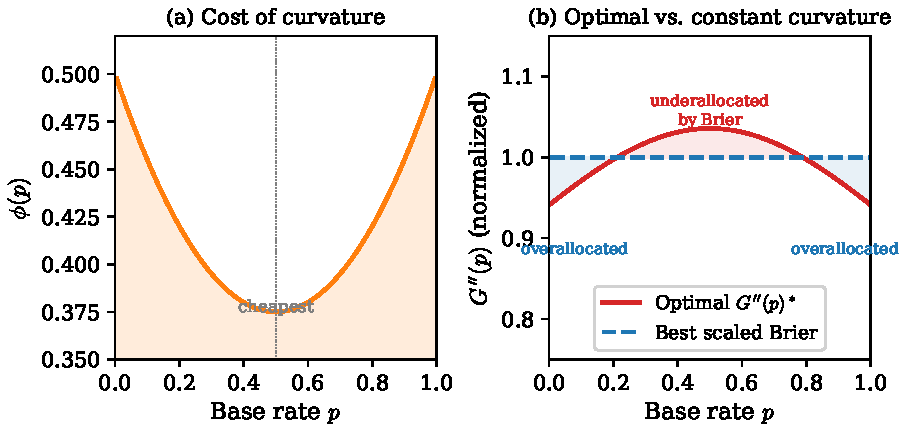
\includegraphics[width=\textwidth]{counterexample_figure.pdf}
  \caption{Counterexample with $u(d,x) = -(d-x)^2$ and uniform prior. 
  (a)~The cost of curvature $\phi(p)$ is U-shaped: adding curvature near $p = 1/2$ 
  is cheapest under limited liability. (b)~Since the principal's sensitivity $|H(p)|$ 
  is constant, the optimal rule concentrates curvature where it is cheap. The Brier 
  score's constant curvature overallocates near the boundaries and underallocates 
  near $p = 1/2$.}
  \label{fig:counterexample}
\end{figure}

\subsection{Boundary behavior}

Under the limited liability constraints~\eqref{eq:boundary}, the cost of curvature $\phi(p)$ remains bounded away from zero at the boundaries: $\phi(0) = \int_0^1 p\,f(p)\,dp = \mathbb{E}[p]$ and $\phi(1) = \int_0^1 (1-p)\,f(p)\,dp = \mathbb{E}[1-p]$, both of which are strictly positive whenever the prior $f$ does not concentrate all mass at a single point. Therefore, provided $|H(p)|\,f(p)$ remains bounded as $p \to 0$ or $p \to 1$, the optimal curvature~\eqref{eq:optimal-curvature} stays finite at the boundaries, and the scoring rule has bounded payments.

\section*{The Boundary problem}

Under the random utility model, the agent selects a report $\hat{p}$ to maximize their expected score perturbed by linear noise:
$$\max_{\hat{p}} V_p(\hat{p}) + \theta \hat{p}, \quad \theta \sim N(0, \sigma^2)$$

Applying a first-order Taylor expansion to the first-order condition yields the unconstrained optimal report:
$$\hat{p}_{raw} \approx p - \frac{\theta}{V_p''(p)} = p + \frac{\theta}{G''(p)}$$

Because the Gaussian noise $\theta$ has infinite support, there is a strictly positive probability that $\hat{p}_{raw} \notin [0,1]$ for any base rate $p \in (0,1)$ and noise level $\sigma > 0$. This violates the fundamental requirement that the agent's report must be a valid probability.

\subsection*{Solution: Clipping}

To resolve this, we explicitly constrain the agent's action space to the valid probability interval $[0, 1]$. Because $S$ is a strictly proper scoring rule, the expected score $V_p(\hat{p})$ is strictly concave in $\hat{p}$. The addition of the linear noise term $\theta\hat{p}$ preserves this strict concavity.

For a strictly concave objective function maximized over a closed interval, if the exact unconstrained maximum $\hat{p}_{exact}$ falls outside the interval, the constrained maximum is the nearest boundary point. The agent's actual report is therefore the clipped value:
\begin{equation}
	\hat{p}_c = \max(0, \min(1, \hat{p}_{exact}))
\end{equation}

We establish that clipping strictly reduces the principal's loss using an exact monotonicity argument, avoiding local Taylor approximations entirely. Let the true probability be $p \in (0,1)$. Because $p$ lies strictly within the valid interval, clipping a report that falls outside $[0,1]$ strictly moves the report closer to $p$:
\begin{equation}
	|\hat{p}_c - p| < |\hat{p}_{exact} - p|
\end{equation}

The principal's utility when acting on a valid report $\hat{p} \in [0,1]$ is $W(\hat{p}) \equiv u(d^*(\hat{p}), p)$. By definition of the decision-matched scoring rule, this is exactly the expected score function $V_p(\hat{p})$ analyzed in Proposition 1. As shown in the proof of Proposition 1, $W(\hat{p})$ has a unique stationary point at $\hat{p} = p$, which is a strict maximum. Consequently, $W(\hat{p})$ is strictly increasing on $[0, p]$ and strictly decreasing on $[p, 1]$. Because clipping an out-of-bounds report strictly moves it closer to $p$ to the nearest valid boundary, it strictly increases $W(\hat{p}_c)$ relative to any mathematically valid report further from the truth, thereby minimizing the principal's exact loss $L(\hat{p}) = u(d^*(p), p) - u(d^*(\hat{p}), p)$ given the bounds.

This guarantees that the principal is always strictly better off under the clipped regime when the unconstrained report violates the boundaries, provided the clipped report remains in the neighborhood where $W$ is concave (which is ensured when $\sigma$ is small relative to $\min(p, 1-p)$).

While clipping guarantees an exact reduction in loss, computing the true expected loss under the clipped distribution is analytically intractable: it requires inverting the nonlinear first-order condition $V_p'(\hat{p}) + \theta = 0$ to obtain $\hat{p}_{exact}(\theta)$ for each noise draw, composing with the clipping and loss functions, and integrating against the Gaussian density---none of which admit closed forms for general $G''$. To optimize the scoring rule, we therefore retain the continuous Taylor approximations for both the agent's error ($\hat{p} - p \approx \frac{\theta}{G''(p)}$) and the principal's loss ($L \approx -\frac{1}{2}H(p)(\hat{p}-p)^2$) to form a surrogate objective function.

Optimizing against this unconstrained analytical surrogate does not establish a strict mathematical bound for the exact clipped loss, nor does it guarantee global optimality in the clipped problem. Clipping differentially benefits lower-curvature rules, which produce higher report variance $\sigma^2/[G''(p)]^2$ and hence more probability mass outside $[0,1]$, creating a larger gap between the surrogate and the true loss. The surrogate therefore serves as a tractable heuristic for allocating curvature, which remains highly accurate in the small-noise regime where boundary reports are rare.

\begin{comment}
\section{Log-odds reparametrization}\label{sec:logodds}

A problem with the model in Section~\ref{sec:random-utility} is that $\hat{p} = p - \theta / V_p''(p)$ can fall outside $(0,1)$ for any $\sigma^2 > 0$, since $\theta$ has unbounded support. Working in log-odds space resolves this. The reparametrization also changes the noise structure: instead of additive noise in probability space, the agent now faces additive noise in log-odds. This is a different model, not merely a change of variables, and the optimal scoring rule will differ accordingly.

\subsection{Transformation}

Define the logit transformation $\operatorname{logit} : (0,1) \to \mathbb{R}$ by
\[
\operatorname{logit}(\hat{p}) = \log \frac{\hat{p}}{1 - \hat{p}},
\]
with inverse $\sigma : \mathbb{R} \to (0,1)$ given by the logistic function
\[
\sigma(\hat{\ell}) = \frac{1}{1 + e^{-\hat{\ell}}}.
\]
Instead of choosing $\hat{p} \in (0,1)$ directly, the agent chooses $\hat{\ell} \in \mathbb{R}$, which maps to the reported probability $\hat{p} = \sigma(\hat{\ell}) \in (0,1)$.

\subsection{Agent's problem in log-odds}

Define $\tilde{V}_p(\hat{\ell}) = V_p(\sigma(\hat{\ell}))$. The agent maximizes
\begin{equation}\label{eq:logodds-obj}
\tilde{V}_p(\hat{\ell}) + \theta \hat{\ell}, \qquad \hat{\ell} \in \mathbb{R}, \quad \theta \sim N(0, \sigma^2).
\end{equation}
Since $\hat{\ell}$ ranges over all of $\mathbb{R}$, the Gaussian noise poses no support problem: for any realization of $\theta$, the optimal $\hat{\ell}^*$ maps to a valid probability $\hat{p} = \sigma(\hat{\ell}^*) \in (0,1)$.

Since $V_p$ is maximized at $\hat{p} = p$ (by properness of $S$) and $\sigma$ is a bijection, $\tilde{V}_p$ is maximized at $\ell = \operatorname{logit}(p)$. The first-order condition for~\eqref{eq:logodds-obj} is $\tilde{V}_p'(\hat{\ell}) + \theta = 0$. Expanding to first order Taylor approximation around $\ell$:
\[
\hat{\ell} \approx \ell - \frac{\theta}{\tilde{V}_p''(\ell)}.
\]

\subsection{Curvature in log-odds}

By the chain rule:
\[
\tilde{V}_p''(\hat{\ell}) = V_p''(\sigma(\hat{\ell})) \cdot [\sigma'(\hat{\ell})]^2 + V_p'(\sigma(\hat{\ell})) \cdot \sigma''(\hat{\ell}).
\]
At $\hat{\ell} = \ell$, the second term vanishes because $V_p'(p) = 0$. Using $\sigma'(\ell) = p(1-p)$:
\begin{equation}\label{eq:curvature-logodds}
\tilde{V}_p''(\ell) = V_p''(p) \cdot p^2(1-p)^2.
\end{equation}

\begin{remark}[Ranking of scoring rules is preserved]
The factor $p^2(1-p)^2$ in \eqref{eq:curvature-logodds} depends only on $p$, not on the scoring rule $S$. Therefore, for a fixed $p$, the ranking of scoring rules by $|\tilde{V}_p''(\ell)|$ is determined entirely by $|V_p''(p)|$, just as in the original model.
\end{remark}

\subsection{Reporting variance in probability space}

To translate the log-odds error back to probability space, expand $\hat{p} = \sigma(\hat{\ell})$ to first order around $\ell$:
\[
\hat{p} - p \approx \sigma'(\ell)(\hat{\ell} - \ell) = p(1-p)(\hat{\ell} - \ell).
\]
Using $\tilde{V}_p''(\ell) = V_p''(p)  \cdot p^2(1-p)^2$ from~\eqref{eq:curvature-logodds} and Remark~\ref{rem:curvature-connection}:
\begin{equation}\label{eq:var-logodds-pspace}
\operatorname{Var}(\hat{p} - p) \approx \frac{p^2(1-p)^2 \,\sigma^2}{[\tilde{V}_p''(\ell)]^2} = \frac{\sigma^2}{[G''(p)]^2 \cdot p^2(1-p)^2}.
\end{equation}
Compared to the probability-space model~\eqref{eq:var-G}, the variance has a factor of $1/[p^2(1-p)^2]$. For a given scoring rule (i.e.\ fixed $G''$), the log-odds model implies higher reporting variance near $p = 0$ and $p = 1$, where the logistic function is flat and the curvature $\tilde{V}_p''(\ell)$ is suppressed relative to $V_p''(p)$.

\subsection{Modified principal's problem}

Since only the variance formula changes, the principal's expected loss~\eqref{eq:expected-loss} becomes:
\begin{equation}\label{eq:expected-loss-logodds}
\mathbb{E}[L \mid p] \approx -\frac{\sigma^2\,H(p)}{2\,[G''(p)]^2\,p^2(1-p)^2}.
\end{equation}
The limited liability constraint remains $S(\hat{p}, x) \geq 0$ in probability space, so the Green's function representation~\eqref{eq:greens} and the payment term are unchanged. The principal's problem is:
\begin{equation}\label{eq:principal-problem-logodds}
\max_{S \in \mathcal{S}} \int_0^1 \left[ \frac{\sigma^2\,H(p)\,f(p)}{2\,[G''(p)]^2\,p^2(1-p)^2} - \alpha\,G(p) \right] f(p)\,dp.
\end{equation}
Writing $g(p) = G''(p) > 0$ and using the separable reformulation from Section~\ref{sec:separable}, the objective becomes:
\begin{equation}\label{eq:separable-logodds}
\int_0^1 \left[ \frac{\sigma^2\,H(p)\,f(p)}{2\,g(p)^2\,p^2(1-p)^2} - \alpha\,\phi(p)\,g(p) \right] dp,
\end{equation}
which is again separable in $g$.

\subsection{Pointwise optimization}

At each $p$, maximize over $g > 0$:
\[
h(g) = \frac{\sigma^2\,H(p)\,f(p)}{2\,g^2\,p^2(1-p)^2} - \alpha\,\phi(p)\,g.
\]
Setting $h'(g) = 0$:
\[
\frac{-\sigma^2\,H(p)\,f(p)}{g^3\,p^2(1-p)^2} = \alpha\,\phi(p),
\]
so that:
\begin{equation}\label{eq:g-cubed-logodds}
g^3 = \frac{\sigma^2\,|H(p)|\,f(p)}{\alpha\,\phi(p)\,p^2(1-p)^2}.
\end{equation}
The second derivative $h''(g) = 3\sigma^2 H(p) f(p) / [g^4 p^2(1-p)^2] < 0$ confirms this is a maximum. The optimal curvature is:
\begin{equation}\label{eq:optimal-curvature-logodds}
\boxed{G''(p)^*_{\text{lo}} = \left( \frac{\sigma^2\,|H(p)|\,f(p)}{\alpha\,\phi(p)\,p^2(1-p)^2} \right)^{1/3}.}
\end{equation}

\subsection{Comparison with the probability-space solution}

The log-odds optimal curvature~\eqref{eq:optimal-curvature-logodds} differs from the probability-space optimal curvature~\eqref{eq:optimal-curvature} by a factor of $[p^2(1-p)^2]^{-1/3}$:
\[
G''(p)^*_{\text{lo}} = \frac{G''(p)^*_{\text{prob}}}{[p^2(1-p)^2]^{1/3}}.
\]
This factor is minimized at $p = 1/2$, where it equals $2^{4/3} \approx 2.52$, and diverges as $p \to 0$ or $p \to 1$. The log-odds model therefore demands more curvature everywhere, and substantially more near the boundaries, than the probability-space model does.

In the log-odds model, the noise $\theta$ perturbs the agent's choice in $\hat{\ell}$-space. Near $p = 0$ or $p = 1$, the logistic map $\sigma$ is flat, so the curvature of $V_p$ in probability space translates to a much weaker curvature $\tilde{V}_p''(\ell) = V_p''(p) \cdot p^2(1-p)^2$ in log-odds space. The optimal scoring rule compensates by increasing $G''(p)$ near the boundaries.

\subsection{Boundary behavior}

Unlike the probability-space solution, $G''(p)^*_{\text{lo}}$ diverges as $p \to 0$ or $p \to 1$. Near $p = 0$, if $|H(p)|\,f(p)/\phi(p)$ has a finite limit, then $G''(p)^*_{\text{lo}} \sim C \cdot p^{-2/3}$ for some constant $C > 0$.

Despite this divergence, the scoring rule has bounded payments. The Green's function representation gives $G(p) = \int_0^1 K(p,t)\,g(t)\,dt$. For any fixed $p \in (0,1)$ and $t$ near $0$, we have $t < p$, so the relevant kernel branch is $K(p,t) = p(1-t) \to p$. Combined with $g(t) \sim t^{-2/3}$, the integrand behaves like $p \cdot t^{-2/3}$, which is integrable since $\int_0^\epsilon t^{-2/3}\,dt = 3\epsilon^{1/3} < \infty$. By symmetry, integrability also holds near $t = 1$. Therefore $G(p) < \infty$ for all $p \in [0,1]$.

For $G'(p)$: since $G'(p) = G'(0) + \int_0^p g(t)\,dt$ and $\int_0^p t^{-2/3}\,dt = 3p^{1/3} < \infty$, the derivative is also finite. The scoring rule payments $S(\hat{p}, 1) = G(\hat{p}) + (1-\hat{p})\,G'(\hat{p})$ and $S(\hat{p}, 0) = G(\hat{p}) - \hat{p}\,G'(\hat{p})$ are therefore bounded and non-negative (the boundary conditions ensure $S(0,1) = S(1,0) = 0$).

\subsection{When is $S_u$ optimal in the log-odds model?}

For $S_u$, we have $G''(p) = |H(p)|$. Substituting into~\eqref{eq:optimal-curvature-logodds}:
\[
|H(p)|^3 = \frac{\sigma^2\,|H(p)|\,f(p)}{\alpha\,\phi(p)\,p^2(1-p)^2} \implies |H(p)|^2 = \frac{\sigma^2\,f(p)}{\alpha\,\phi(p)\,p^2(1-p)^2}.
\]
So $S_u$ is optimal if and only if $|H(p)|^2\,\phi(p)\,p^2(1-p)^2 / f(p)$ is constant in $p$. The probability-space condition requires $|H(p)|^2\,\phi(p)/f(p) = \text{const}$, while the log-odds condition requires $|H(p)|^2\,\phi(p)\,p^2(1-p)^2/f(p) = \text{const}$. These two conditions are generically incompatible: if the first holds, the second equals a constant times $p^2(1-p)^2$, which is not constant; if the second holds, the first equals a constant times $1/[p^2(1-p)^2]$, which is not constant. So the two models impose different constraints on when $S_u$ is optimal.

\subsection{Counterexample revisited}

Take $u(d,x) = -(d-x)^2$ and $f(p) = 1$ as in Section~7.7. Then $H(p) = -2$, $\phi(p) = (p^2 - p + 1)/2$, and:
\begin{equation}\label{eq:logodds-counterexample}
G''(p)^*_{\text{lo}} = \left( \frac{4\sigma^2}{\alpha\,(p^2 - p + 1)\,p^2(1-p)^2} \right)^{1/3}.
\end{equation}
This diverges at the boundaries, in contrast to the probability-space solution which was finite everywhere. The Brier score (constant curvature $G'' = 2$) now underallocates curvature not only near $p = 1/2$ (as in the probability-space model) but also, and much more severely, near the boundaries $p \approx 0$ and $p \approx 1$.

\subsection{Which model should be preferred?}
In the probability-space model, the noise term $\varepsilon(\hat{p}) = \theta\hat{p}$ has larger absolute values for reports near $\hat{p} = 1$ than near $\hat{p} = 0$. However, this does not translate into asymmetric reporting errors: since $\varepsilon(\hat{p})$ is linear in $\hat{p}$, its derivative with respect to $\hat{p}$ is simply $\theta$, so the marginal perturbation to the agent's first-order condition is constant across $(0,1)$. The resulting reporting error $\hat{p} - p \approx -\theta / V_p''(p)$ depends only on the curvature of the scoring rule and the noise realization, not on the level of the report. If the scoring rule has constant curvature (like the Brier score), the probability-space model produces uniform error variance everywhere.

The log-odds model has the more natural property that noise is symmetric around the difficulty of the discrimination task: a perturbation of $\Delta\hat{\ell}$ in log-odds has the same effect on the reported probability whether the base rate is $p$ or $1-p$. For a fixed scoring rule, the log-odds model implies that the agent's reporting errors in probability space are \emph{largest} near $p = 0$ and $p = 1$ and \emph{smallest} near $p = 1/2$, as can be seen from~\eqref{eq:var-logodds-pspace}: the factor $1/[p^2(1-p)^2]$ diverges at the boundaries and is minimized at $p = 1/2$. The choice between models is ultimately an empirical question about the structure of forecaster errors.

\newpage
\section{Numerical verification}\label{sec:numerical}

Both the probability-space and log-odds models rely on second-order Taylor approximations to derive tractable variance formulas and optimal curvature profiles. This section validates these approximations numerically, using the counterexample $u(d,x) = -(d-x)^2$ with uniform prior $f \equiv 1$ throughout.

\subsection{Verification of analytical formulas}

We first verify the closed-form expressions from the counterexample (Sections~6.7 and~7.10). Monte Carlo simulation with $n = 500{,}000$ draws confirms:
\begin{itemize}
\item The cost of curvature $\phi(p) = (p^2 - p + 1)/2$ matches the numerical evaluation of \eqref{eq:phi-explicit} to machine precision ($< 10^{-15}$).
\item The principal's sensitivity $H(p) = -2$ is constant, as predicted.
\item The Green's function representation \eqref{eq:greens} with $g \equiv 2$ (Brier score) recovers $G(p) = p^2 - p + 1$ to accuracy $< 10^{-7}$, and the boundary conditions $G(0) + G'(0) = 0$ and $G(1) - G'(1) = 0$ are satisfied.
\item The optimality condition $|H(p)|^2 \phi(p)/f(p) = 2(p^2 - p + 1)$ ranges from $1.5$ to $2.0$, confirming that $S_u$ (the Brier score) is not optimal.
\end{itemize}

\subsection{Properness of $S_u$}

For the quadratic utility, $S_u(\hat{p}, 1) = -(\hat{p} - 1)^2$ and $S_u(\hat{p}, 0) = -\hat{p}^2$. Numerical grid search confirms that $V_p(\hat{p}) = p\,S_u(\hat{p},1) + (1-p)\,S_u(\hat{p},0)$ is uniquely maximized at $\hat{p} = p$ for all tested values $p \in \{0.1, 0.25, 0.5, 0.75, 0.9\}$, consistent with the analytical result $V_p'(\hat{p}) = -2\hat{p} + 2p = 0 \implies \hat{p} = p$ and $V_p'' = -2 < 0$.

\subsection{Probability-space Taylor approximation}\label{sec:num-prob-taylor}

In the probability-space model (Section~\ref{sec:random-utility}), the agent maximizes $V_p(\hat{p}) + \theta\hat{p}$ where $\theta \sim N(0, \sigma^2)$. For the Brier score, the first-order condition yields the closed-form solution $\hat{p} = p + \theta/2$, and the Taylor approximation \eqref{eq:var-phat} predicts $\operatorname{Var}(\hat{p} - p) = \sigma^2/4$.

Table~\ref{tab:prob-taylor} reports Monte Carlo results. The Taylor approximation is accurate to within $5\%$ for $\sigma \leq 0.1$ across all base rates, including near the boundaries. The only deviations (${\sim}4\%$) occur at $p \in \{0.1, 0.9\}$ with $\sigma = 0.1$, where the clipping of $\hat{p}$ to $[0,1]$ becomes noticeable.

\begin{table}[h]
\centering
\caption{Probability-space model: relative error $(\operatorname{Var}_{\text{MC}} - \operatorname{Var}_{\text{Taylor}})/\operatorname{Var}_{\text{Taylor}}$ for the Brier score.}
\label{tab:prob-taylor}
\begin{tabular}{r|rrrrr}
$\sigma$ & $p=0.1$ & $p=0.3$ & $p=0.5$ & $p=0.7$ & $p=0.9$ \\
\hline
0.01 & $+0.002$ & $+0.000$ & $-0.002$ & $-0.001$ & $+0.001$ \\
0.05 & $-0.002$ & $+0.001$ & $+0.000$ & $-0.005$ & $+0.001$ \\
0.10 & $-0.038$ & $-0.001$ & $-0.001$ & $-0.001$ & $-0.042$ \\
\end{tabular}
\end{table}

For the log score ($G''(p) = 1/[p(1-p)]$), the Taylor approximation $\operatorname{Var}(\hat{p} - p) \approx \sigma^2 p^2(1-p)^2$ is similarly accurate, with relative errors below $5\%$ for $\sigma \leq 0.1$.

\subsection{Log-odds Taylor approximation}\label{sec:num-logodds-taylor}

In the log-odds model (Section~\ref{sec:logodds}), the agent maximizes $\tilde{V}_p(\hat{\ell}) + \theta\hat{\ell}$ over $\hat{\ell} \in \mathbb{R}$. The Taylor approximation \eqref{eq:var-logodds-pspace} predicts $\operatorname{Var}(\hat{p} - p) \approx \sigma^2 / [G''(p)^2 \, p^2(1-p)^2]$.

Numerical verification reveals a fundamental issue: for the Brier score, the agent's first-order condition
\begin{equation}\label{eq:brier-foc-logodds}
2(p - \sigma(\hat{\ell})) \cdot \sigma(\hat{\ell})(1 - \sigma(\hat{\ell})) + \theta = 0
\end{equation}
does not always have an interior solution. The left-hand side (excluding $\theta$) is bounded: define
\[
\tilde{V}_p'(\hat{\ell}) = 2(p - \sigma(\hat{\ell})) \cdot \sigma(\hat{\ell})(1 - \sigma(\hat{\ell})),
\]
which satisfies $\tilde{V}_p'(\hat{\ell}) \to 0$ as $\hat{\ell} \to \pm\infty$ (since $\sigma \to 0$ or $1$). Therefore $|\tilde{V}_p'|$ achieves a finite maximum, and for $|\theta|$ exceeding this maximum, the equation \eqref{eq:brier-foc-logodds} has no solution. In this case, the agent's objective $\tilde{V}_p(\hat{\ell}) + \theta\hat{\ell}$ is monotone in $\hat{\ell}$, and the agent's optimal report is a boundary value: $\hat{p} \in \{0, 1\}$.

\begin{table}[h]
\centering
\caption{Maximum incentive gradient $\max_{\hat{\ell}} |\tilde{V}_p'(\hat{\ell})|$ and probability of boundary reports for the Brier score in the log-odds model.}
\label{tab:boundary-reports}
\begin{tabular}{r|cccc}
 & $p = 0.05$ & $p = 0.1$ & $p = 0.3$ & $p = 0.5$ \\
\hline
$\max |\tilde{V}_p'|$ & $0.001$ & $0.005$ & $0.039$ & $0.096$ \\[4pt]
\multicolumn{5}{l}{$\Pr(\text{boundary report})$:} \\
$\sigma = 0.01$ & $45.2\%$ & $31.7\%$ & $0.0\%$ & $0.0\%$ \\
$\sigma = 0.05$ & $49.0\%$ & $46.2\%$ & $22.1\%$ & $5.4\%$ \\
$\sigma = 0.10$ & $49.8\%$ & $48.7\%$ & $39.5\%$ & $33.6\%$ \\
$\sigma = 0.50$ & $79.1\%$ & $80.3\%$ & $83.7\%$ & $84.7\%$ \\
\end{tabular}
\end{table}

This explains the Taylor approximation's breakdown in the log-odds model. The approximation assumes the agent's response is locally linear around the truth, but for a significant fraction of noise draws, the agent is driven to a corner solution instead. Table~\ref{tab:boundary-reports} quantifies this: even at $\sigma = 0.01$, boundary reports occur for $45\%$ of draws at $p = 0.05$ and $32\%$ at $p = 0.1$.

The phenomenon is not specific to the Brier score. Any scoring rule with bounded payments satisfies $S(\hat{p}, x) \in [0, M]$ for some $M < \infty$, which implies $\tilde{V}_p'(\hat{\ell}) \to 0$ as $\hat{\ell} \to \pm\infty$ and hence a bounded incentive gradient. The critical quantity is the \emph{effective noise ratio}:
\begin{equation}\label{eq:effective-noise}
\rho(p) \equiv \frac{\sigma}{\max_{\hat{\ell}} |\tilde{V}_p'(\hat{\ell})|}.
\end{equation}
The Taylor approximation is reliable when $\rho(p) \ll 1$, i.e., when the noise is small relative to the maximum incentive the scoring rule can provide. For the Brier score, $\max |\tilde{V}_p'| \approx 2p^2(1-p)^2$ near the boundaries, so $\rho(p) \to \infty$ as $p \to 0$ or $p \to 1$ regardless of $\sigma$.

\subsubsection{Comparison with the log score}

The log score avoids this problem because its payments are unbounded: $S(\hat{p}, 1) = \ln \hat{p} \to -\infty$ as $\hat{p} \to 0$. In the log-odds model, the log score objective is globally concave:
\[
\tilde{V}_p(\hat{\ell}) + \theta\hat{\ell} = (p + \theta)\hat{\ell} - \ln(1 + e^{\hat{\ell}}) + \text{const},
\]
which is strictly concave in $\hat{\ell}$ with a unique interior maximum at $\sigma(\hat{\ell}) = p + \theta$ whenever $p + \theta \in (0,1)$. The closed-form solution $\hat{p} = p + \theta$ shows that the Taylor approximation for the log score is exact (not merely approximate) in the log-odds model. Boundary reports occur only when $|{\theta}| > \min(p, 1-p)$, which for $p = 0.5$ requires $\sigma > 0.5$.

\subsection{Optimal curvature comparison}

Table~\ref{tab:principal-gain} compares the principal's net utility under the optimal curvature profile \eqref{eq:optimal-curvature} versus the best-scaled Brier score, both evaluated using the Taylor-approximated loss in the probability-space model. The optimal rule provides a consistent $0.18\%$ improvement across noise levels, reflecting the modest non-uniformity of $\phi(p)$ in the quadratic-uniform counterexample.

\begin{table}[h]
\centering
\caption{Principal's net utility (probability-space model, $\alpha = 1$).}
\label{tab:principal-gain}
\begin{tabular}{r|ccc}
$\sigma^2$ & Optimal & Brier (scaled) & Improvement \\
\hline
$0.01$ & $-0.2216$ & $-0.2220$ & $+0.18\%$ \\
$0.10$ & $-0.4775$ & $-0.4783$ & $+0.18\%$ \\
$1.00$ & $-1.0287$ & $-1.0305$ & $+0.18\%$ \\
\end{tabular}
\end{table}

\subsection{Implications for the log-odds model}\label{sec:logodds-implications}

The numerical findings reveal that the log-odds model with additive noise $\theta\hat{\ell}$ imposes a compatibility requirement on the scoring rule: the payments must grow fast enough at the boundaries to prevent the linear noise term from dominating the incentive gradient. Specifically:
\begin{itemize}
\item \textbf{Bounded scoring rules} (including Brier and the optimal rule \eqref{eq:optimal-curvature-logodds}, whose curvature diverges as $p^{-2/3}$ but whose payments remain bounded) produce boundary reports for a positive fraction of noise draws at every $\sigma > 0$. The Taylor approximation is unreliable in this regime.
\item \textbf{Unbounded scoring rules} (such as the log score, with $G''(p) = 1/[p(1-p)]$) maintain interior solutions for a much wider range of noise levels, and the Taylor approximation can be exact (as for the log score).
\end{itemize}

Several approaches can address this issue:
\begin{enumerate}
\item \textbf{Small-noise regime.} Restrict attention to $\sigma$ small enough that boundary reports are rare. The Taylor approximation is valid when $\rho(p) \ll 1$, i.e., $\sigma \ll \max_{\hat{\ell}} |\tilde{V}_p'(\hat{\ell})|$. The resulting optimal curvature \eqref{eq:optimal-curvature-logodds} remains a valid local approximation in this regime, even though it does not capture the global behavior of the agent's problem.
\item \textbf{Optimize within unbounded-payment families.} Restrict the optimization to scoring rules with payments that grow sufficiently fast at the boundaries (e.g., $G''(p) \sim [p(1-p)]^{-\beta}$ with $\beta \geq 1$). These rules maintain well-behaved agent optima for larger noise levels. The optimization over $\beta$ and the scale parameter can be performed numerically using exact Monte Carlo evaluation of the expected loss.
\item \textbf{Model boundary reports explicitly.} When $|\theta| > \max |\tilde{V}_p'|$, the agent reports $\hat{p} \in \{0,1\}$. The exact expected loss includes these corner solutions and can be computed numerically. This leads to a non-smooth optimization problem that no longer admits a closed-form solution but can be solved computationally.
\item \textbf{Use the probability-space model as the primary framework.} The probability-space Taylor approximation works well (Section~\ref{sec:num-prob-taylor}), and the support issue ($\hat{p}$ leaving $[0,1]$) can be handled by clipping. The log-odds model then serves as a robustness check for the qualitative conclusions about curvature allocation.
\end{enumerate}
\end{comment}
\newpage

\section*{Notes for continuation}
\textbf{Status.} Sections 1--6 set up the model: we define the principal-agent problem, the decision-matched scoring rule $S_u$, prove properness, introduce the random utility model with Gaussian noise, and formulate the principal's optimization problem. Section~\ref{sec:limited-liability} solves the optimal scoring rule under limited liability ($S \geq 0$), yielding a closed-form solution for optimal curvature \eqref{eq:optimal-curvature}. Section~7 reparametrizes the agent's problem in log-odds, resolving the unbounded-support issue of the probability-space model, and derives the corresponding optimal curvature \eqref{eq:optimal-curvature-logodds}.

\textbf{Key results so far.}
\begin{itemize}
\item The limited liability constraint $S(\hat{p}, x) \geq 0$ reduces to $G(0) + G'(0) \geq 0$ and $G(1) - G'(1) \geq 0$, both of which bind at optimum.
\item With boundary conditions $G(0) + G'(0) = 0$ and $G(1) - G'(1) = 0$, $G$ is expressed via a Green's function \eqref{eq:greens} as a linear functional of $g = G''$.
\item The principal's problem becomes separable in $g$, which enables pointwise optimization.
\item \textbf{Probability-space model:} the optimal curvature is $G''(p)^* = \left(\sigma^2 |H(p)| f(p) / (\alpha \phi(p))\right)^{1/3}$. $S_u$ is optimal if and only if $|H(p)|^2 \phi(p) / f(p)$ is constant in $p$.
\item \textbf{Log-odds model:} the optimal curvature is $G''(p)^*_{\mathrm{lo}} = \left(\sigma^2 |H(p)| f(p) / (\alpha \phi(p) p^2(1-p)^2)\right)^{1/3}$. This diverges as $p \to 0$ or $p \to 1$, but the scoring rule retains bounded payments because $g(t) \sim t^{-2/3}$ is integrable against the Green's function kernel. The two models impose generically incompatible conditions for $S_u$ optimality: the probability-space model requires $|H(p)|^2 \phi(p) / f(p) = \text{const}$, while the log-odds model requires $|H(p)|^2 \phi(p) p^2(1-p)^2 / f(p) = \text{const}$.
\item In the counterexample ($u(d,x) = -(d-x)^2$, $f \equiv 1$), both models show that the Brier score's constant curvature is suboptimal: it underallocates curvature near $p = 1/2$ (where curvature is cheapest under limited liability) and, in the log-odds model, also severely underallocates near the boundaries.
\item \textbf{Numerical verification} (Section~\ref{sec:numerical}): the probability-space Taylor approximation is accurate to within $5\%$ for $\sigma \leq 0.1$. The log-odds model has a fundamental compatibility issue: bounded scoring rules produce boundary reports ($\hat{p} \in \{0,1\}$) for a positive fraction of noise draws, because the incentive gradient $\tilde{V}_p'(\hat{\ell})$ is bounded while the noise $\theta$ is not. This invalidates the Taylor approximation for bounded rules at non-negligible noise levels. Section~\ref{sec:logodds-implications} outlines four approaches to address this.
\end{itemize}

\textbf{Open questions and next steps.}
\begin{enumerate}
\item \textbf{Log-odds model resolution.} The numerical verification (Section~\ref{sec:logodds-implications}) identifies four approaches to the boundary-report issue: (i) restrict to the small-noise regime, (ii) optimize within unbounded-payment families, (iii) model boundary reports explicitly, or (iv) use the probability-space model as the primary framework. A decision on which approach to pursue is needed.
\item \textbf{Tail probability of errors.} For any error threshold $\delta > 0$, calculate the probability $\Pr(|\hat{p} - p| > \delta)$ under a given scoring rule $S$. Investigate how this tail probability varies across scoring rules and base rates $p$, under both models.
\item \textbf{Expected gain for the principal.} Compute how the principal's expected gain changes under different scoring rules, assuming a uniform prior $p \sim U[0,1]$. A baseline scenario to model is whether a principal, when facing a forecasting problem themselves, optimally assigns the exact same scoring rule they face to the subcontracted agent.
\item \textbf{Wager extension.} The limited liability constraint models tournament-style platforms like Metaculus, where forecasters cannot lose. For prediction markets, the agent puts up a stake $W$ and can lose money: the constraint becomes $S(\hat{p}, x) \geq -W$ with a participation constraint $G(p) \geq 0$. Derive the optimal curvature under these constraints.
\item \textbf{Empirical model selection.} The probability-space and log-odds models make different predictions about the structure of forecaster errors. Empirical evidence on forecaster calibration would help distinguish between the models.
\end{enumerate}

\end{document}